\documentclass[a4paper]{article}
\usepackage{tikz}
\usepackage{amsmath}
\title{Acrobot}
\begin{document}
\maketitle
\begin{figure}[h]
\centering
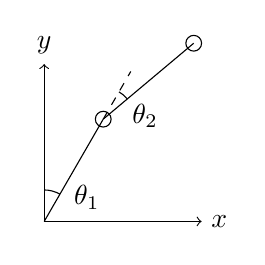
\begin{tikzpicture}
\draw[->] (0,0) -- (2,0) node[anchor=west] {$x$};
\draw[->] (0,0) -- (0,2) node[anchor=south] {$y$};

\draw (0,.4) arc(90:60:.4);
\draw (50:.4) node[anchor=west] {$\theta_1$};
\draw (0,0) -- (60:1.5) circle(.1);
\draw[dashed] (60:1.5) -- +(60:.7);
\draw (60:1.9) arc(60:40:.4);
\draw (60:1.5) +(10:.25) node[anchor=west] {$\theta_2$};
\draw (60:1.5) -- +(40:1.5) circle(.1);
\end{tikzpicture}
\end{figure}

Position
\begin{eqnarray*}
x_1 &=& \sin(\theta_1)\\
y_1 &=& \cos(\theta_1)\\
\end{eqnarray*}
\begin{eqnarray*}
x_2 &=& \sin(\theta_1) + \sin(\theta_1 + \theta_2)\\
y_2 &=& \cos(\theta_1) + \cos(\theta_1 + \theta_2)
\end{eqnarray*}

Kinetic energy
\begin{eqnarray*}
T &=&\frac{1}{2} m_1 \dot{\theta}_1^2 + \frac{1}{2} m_2 \dot{\theta}_1^2
+ \frac{1}{2} m_2 (\dot{\theta}_1 + \dot{\theta_2})^2\\
&&+ m_2 \dot{\theta}_1(\dot{\theta}_1 + \dot{\theta}_2)
\left(\sin(\theta_1)\sin(\theta_1+\theta_2) + \cos(\theta_1)\cos(\theta_1+\theta_2)\right)\\
&=& \frac{1}{2} m_1 \dot{\theta}_1^2 + \frac{1}{2} m_2 \dot{\theta}_1^2
+ \frac{1}{2} m_2 (\dot{\theta}_1 + \dot{\theta_2})^2
+ m_2 \dot{\theta}_1(\dot{\theta}_1 + \dot{\theta}_2) \cos(\theta_2)\\
&=& (\frac{1}{2} m_1 + m_2 + m_2 \cos{\theta_2}) \dot{\theta}_1^2
+ m_2 (1 + \cos{\theta_2}) \dot{\theta}_1 \dot{\theta}_2
+ \frac{1}{2} m_2 \dot{\theta}_2^2\\
&=& \frac{1}{2}
\begin{pmatrix} \dot{\theta}_1 & \dot{\theta}_2 \end{pmatrix}\
\begin{pmatrix} m_1 + 2 m_2 (1 + \cos{\theta_2}) & m_2 (1 + \cos{\theta_2})\\
                m_2 (1 + \cos{\theta_2}) & m_2  \end{pmatrix}
\begin{pmatrix} \dot{\theta}_1\\ \dot{\theta}_2 \end{pmatrix}
\end{eqnarray*}

Potential energy
\begin{eqnarray*}
V &=& m_1 g y_1 + m_2 g y_2\\
  &=& (m_1 + m_2) g \cos{\theta_1} + m_2 g \cos(\theta_1 + \theta_2)
\end{eqnarray*}
\end{document}
